\section{Mail template}
\label{a:mail}
\lstset{language=HTML}
\begin{lstlisting}
<html>
  <head>
    <title>Anti Phishing Education</title>
  </head>
  <body>
    <p>Dies ist eine automatisch generierte E-Mail im Rahmen einer Anti-Phishing Education App. Falls diese nicht angefordert wurde, bitte ignorieren.</p>
    <p>Ansonsten geht es hier weiter:</p>
    <p>Wie du im Absender siehst, hast du dir gerade selbst eine E-Mail mit gef\"{a}lschtem Absender geschickt. Hier ist au{\ss}erdem dein Freitext:</p>
    <p>{$usermessage}</p>
    <p>F\"{u}r einen Angreifer ist es ebenso einfach automatisierte E-Mails mit gef\"{a}lschtem Absender und Inhalt zu verschicken. Meist enthalten diese einen Link zu einer Webseite, genau wie diese E-Mail.</p>
    <p>Um mit der App fortzufahren, klicke auf den folgenden Link.</p>
    <p><a href="http://pages.no-phish.de/maillink.php">http://www.google.com</a></p>
    <p>Viele Gr\"{u}{\ss}e,</p>
    <p>Dein NoPhish Team</p>
  </body>
</html>
\end{lstlisting}

%===========================================
\section{URL Generation}
\label{s:url_generation}
%===========================================
While playing the app the user is presented with URLs that he has to categorize as phish or valid.
While reviewing the previous works and games in this area we found that many of them use a fixed set of examples.
On some games this set is very small and therefore you are always confronted with the same URLs.
As we layed out in Section \autoref{s:url_structure} we want to teach the user how to detect phishing URLs in general.
To accomplish this goal we think that it is essential that the user sees as much different URLs as possible so he can build his own mental model.
Therefore we decided on generating URLs rather than composing a fixed list.
We will lay out the general process here and cover interesting parts of it in the following sections.
\subsection{Example URLs}
To present attacked URLs to the user we found int most realistic to take valid URLs and apply attacks on them.
Therefore we needed a set of valid URLs.
To build this set we used Alexa~\cite{alexa} to find the top 100 domains for german users.
We then went to each of these sites and by navigating tried to find 6 URLs for each domain.
We tried to find some short and some long URLs.
\begin{description}[leftmargin=0cm]
\item[generate attacks for level]When starting a new level we generate a list of Attacks that we want to show the user.
\item[select valid URL]When we want to show a new URL to the user we first randomly select a valid URL from the before mentioned set.
\item[apply generator]Then we apply a generator to the URL that does not invalidate the URL but modifies it.
\item[apply attack]After that we select a random attack from the previously build list and apply it to the URL.
\item[repeat]In some situations we need to try again.
\end{description}
\subsection{generate attacks for level}
\textbf{Was zur historie?}
The types of URLs the user is presented is dependent on the level.
Each level introduces on or more attacks.
Which attack is introduced in which level is layed out in section\autoref{s:knowledgetransferperlevel}.
In general the URLs of each level $n$ are distributed as follows:
\begin{table}[hHtbp]
\centering
\begin{tabular}{llll}
Total number of URLs&$u$&$6+2*n$&starting with 6 URLs each level has 2 more URLS.\\
Number of Phishes&$p$&$u/2$&Half of the URLs are phishes.\\
Number of repeats&$r$&$\left\lfloor p/2 \right\rfloor$&Half of the phishes are repeats.
\end{tabular}
\caption{distribution of URLs per level.}
\label{t:levelurls}
\end{table}

The repeats are always one attack from each previous level. The rest of the repeats is filled up randomly.

There are two main exception to these rules:
\begin{description}[leftmargin=0cm]
\item[Level 1] In Level 1 the game is modified in the form that the user is only presented with valid URLs and has to select the domain.
To prevent boring the user in this level we only present 5 URLs.
None of them is a phish.
\item[Level 1+2] The first level that contain repeats is level 3 because level 2 is the first real game level.
\end{description}

The generated list of attacks also contains a special attack that does no real attack. This is to simplify the URL generation. When we generated the list of attacks we save it for later reference.
\subsection{Apply Generator}
We were unsure if we still have enough valid URLs so we prepared a way to automatically modify the URLs in such a way that they could still be valid URLs. Some Ideas where to add subdomains or path strings to the URL. Query or fragments are also possible. We later found out that it is currently not needed to implement generators because there are a lot of URLs in our set. If however we will some time in the future find out that these URLs are not enough we have this scheme in place.
\subsection{Apply Attack}
After we generated a valid URL we chose a random attack from the previously build set of attacks and apply it to the URL. With this we also store which attack we currently applied. This is important when the user is failing this round. In this situation we will simply readd this attack to the set of attacks.
\subsection{Repeat}
There are combinations of base-URL and attack where the attack doe's not alter the URL.
Therefore it would be impossible for the user to detect the Attack and he will be confused and might stop using the app.
In this situation we repeat the whole URL generation process until we find a matching URL.

\section{Presurvey Form}
\label{s:presurvey_form}
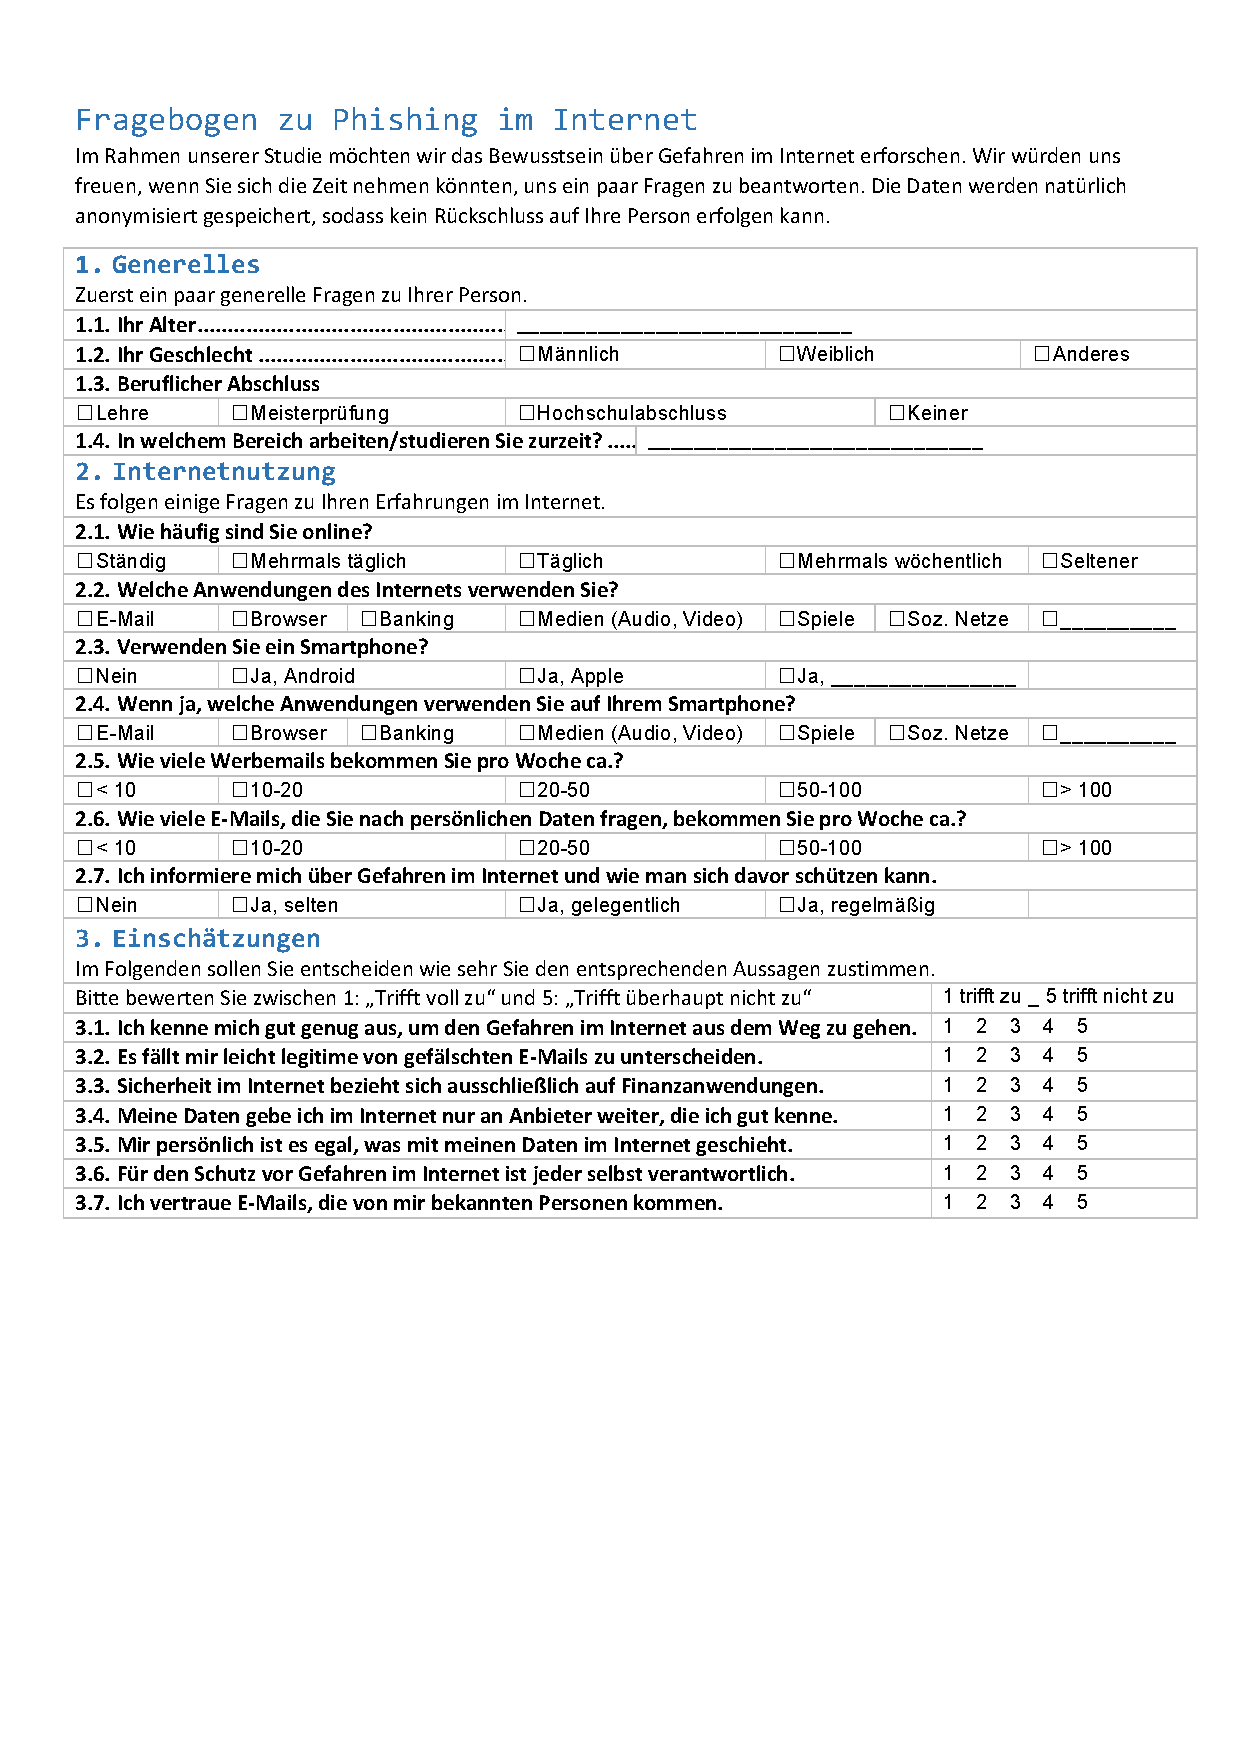
\includepdf[pages=-,frame,scale=0.8]{graphix/presurvey.pdf}

\section{Study Forms}
The following pages contain the forms as we used them in the user study. We did not include all example URL but only one exemplary page with an attacked URL.
\label{s:before_survey}
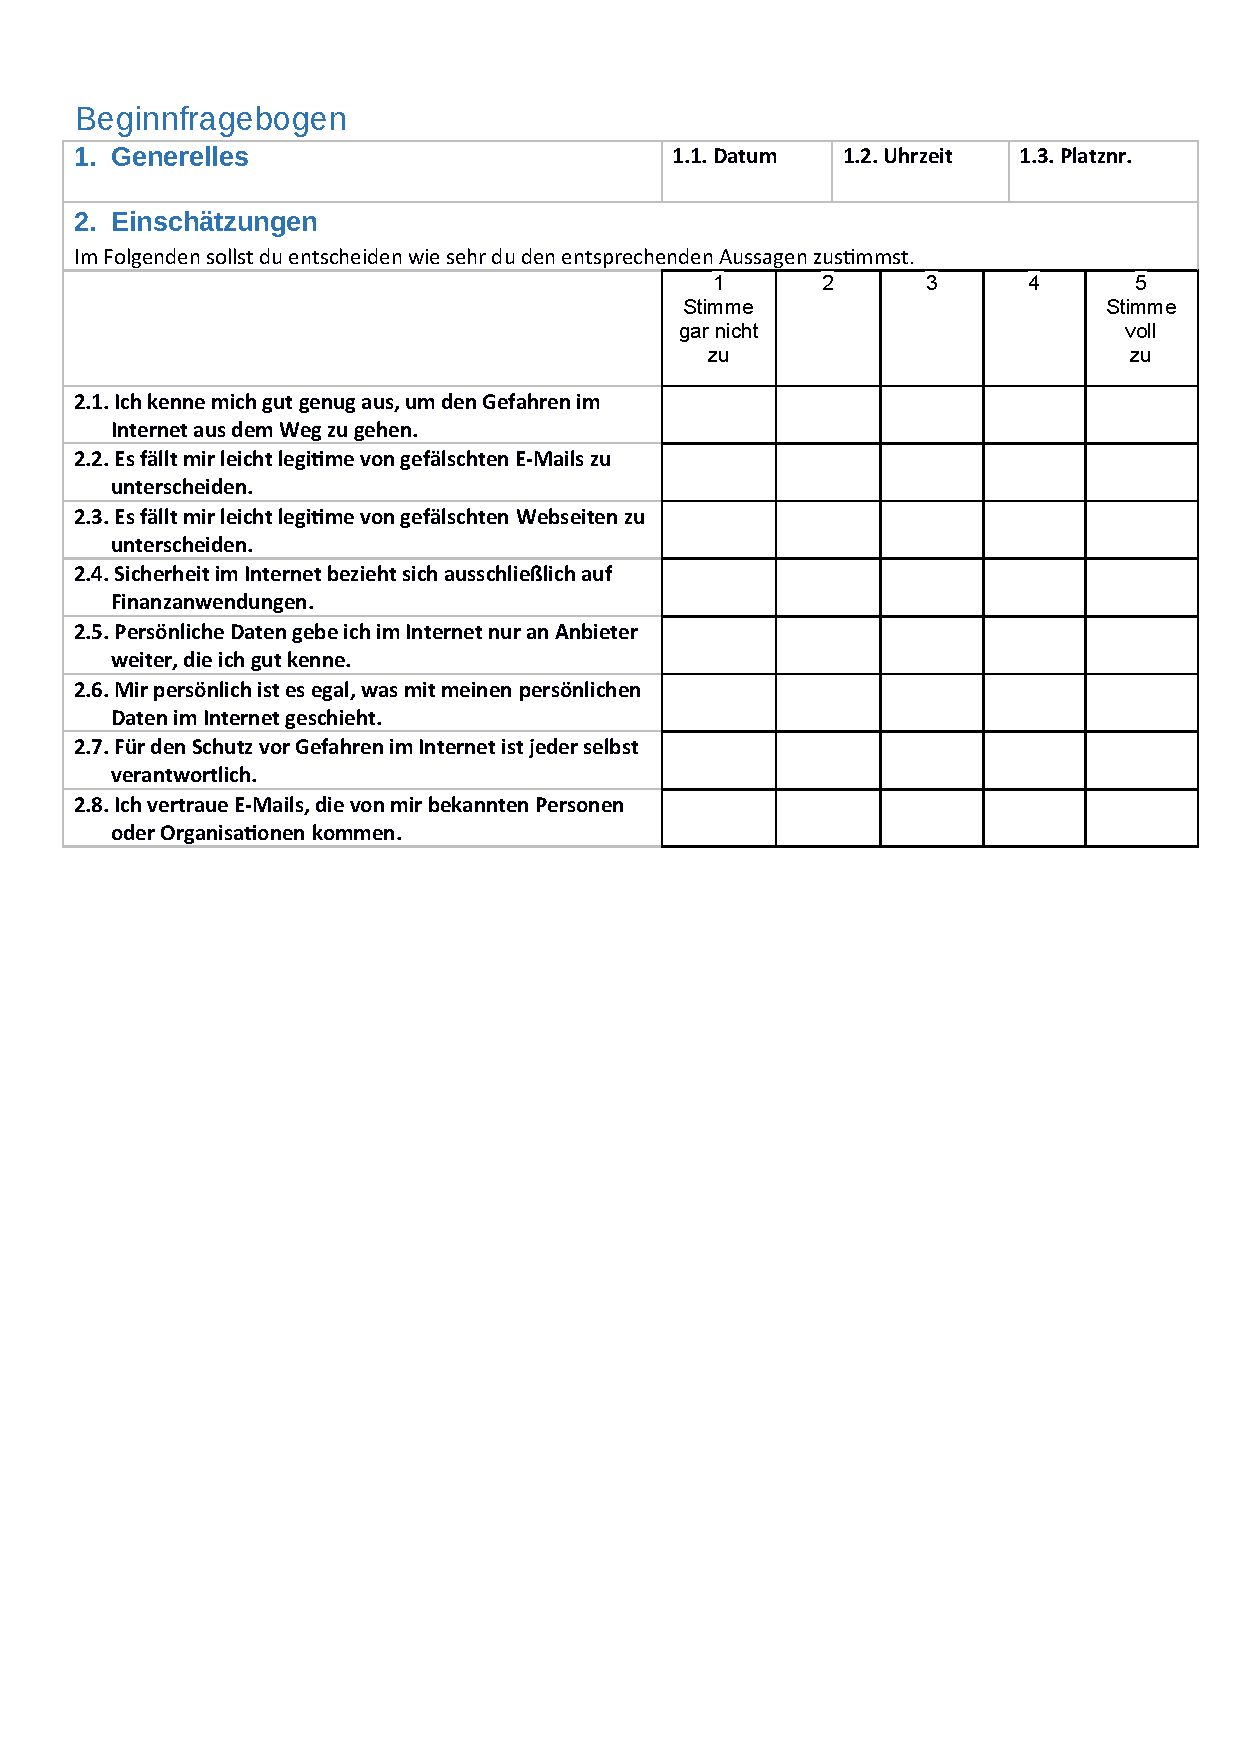
\includepdf[pages=-,frame,scale=0.8]{graphix/before_survey.pdf}
\label{s:url_survey}
\includepdf[pages={1,10},frame,scale=0.8]{graphix/url_survey.pdf}
\label{s:after_survey}
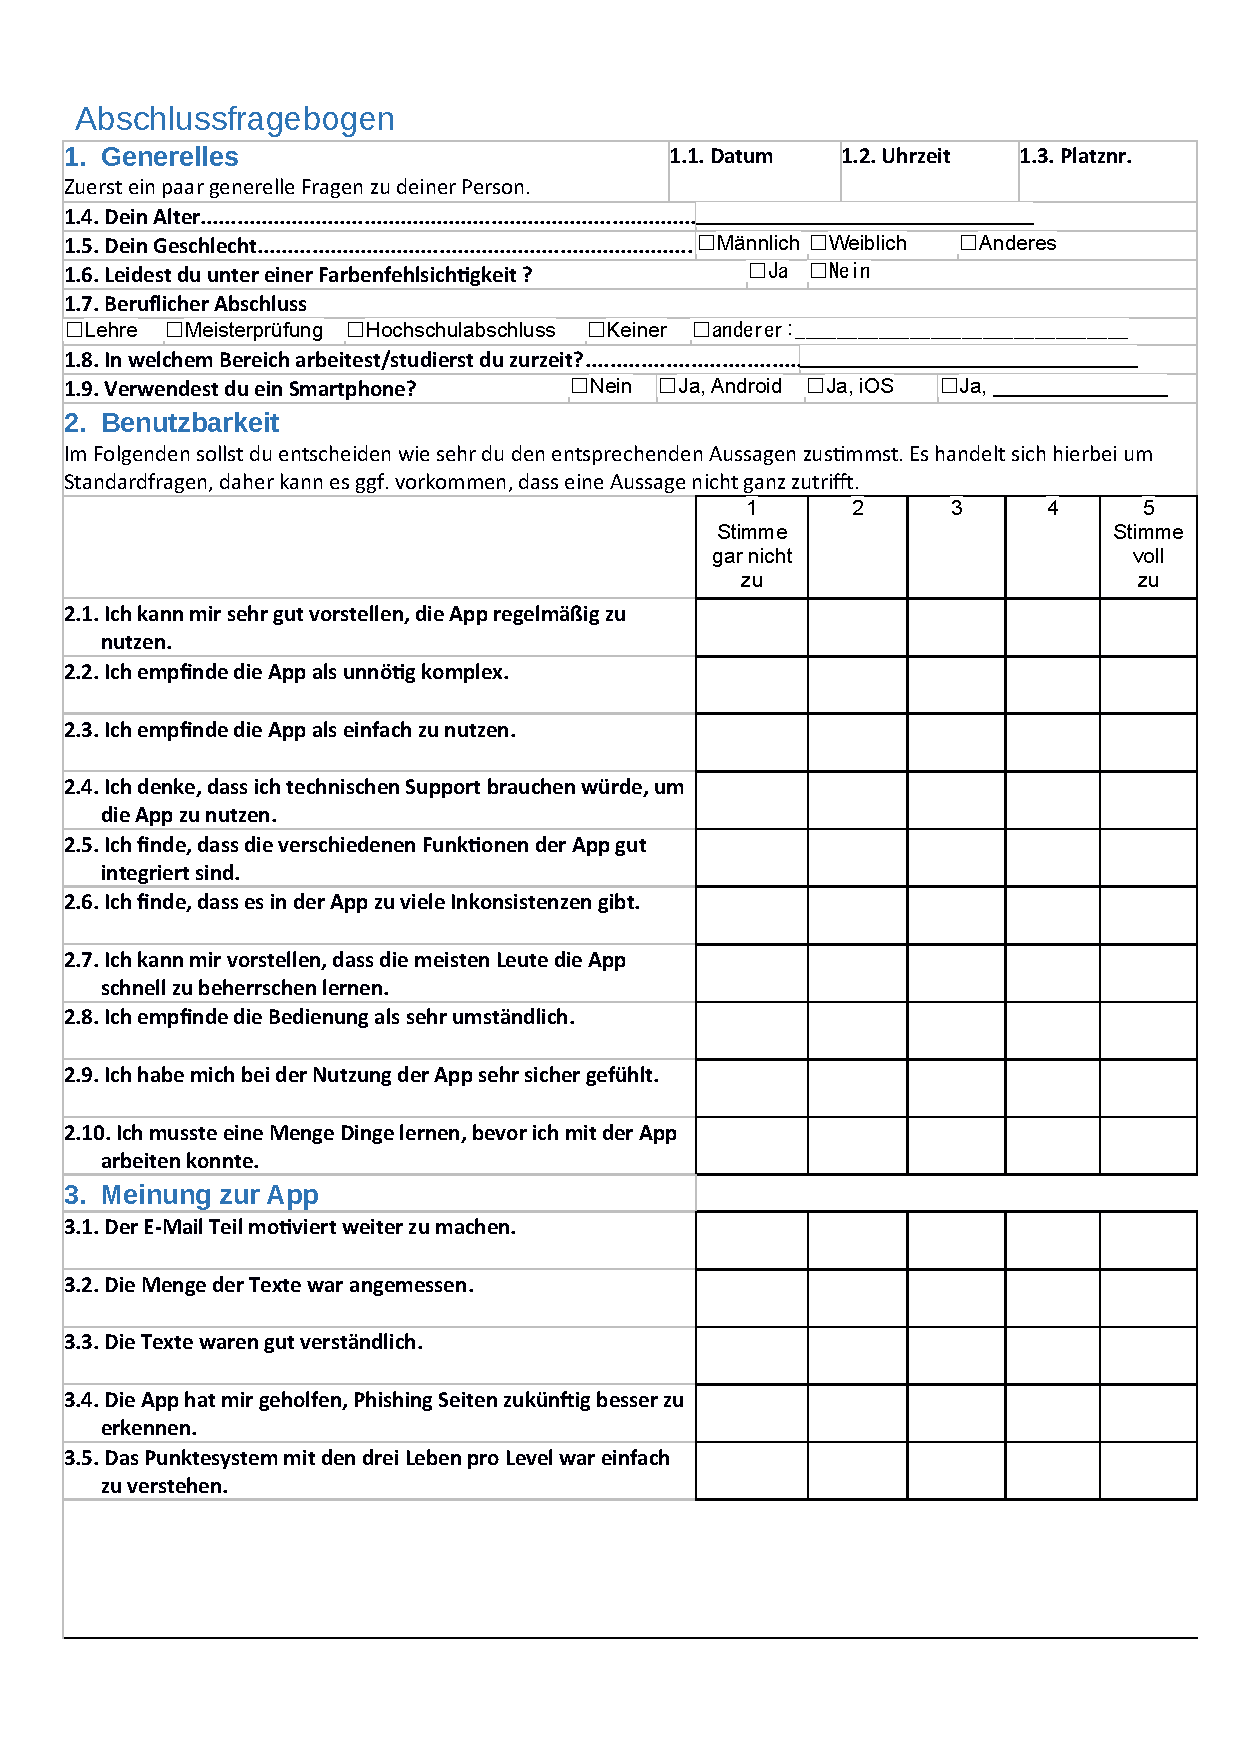
\includepdf[pages={1},frame,scale=0.8]{graphix/after_survey.pdf}

\section{Participant Recruitment for User Study}
\label{s:participant_recruitment}

Sehr geehrte/r ....,

wir, Clemens Bergmann und Gamze Canova, sind Studenten des Fachbereichs Informatik an der TU Darmstadt und arbeiten zur Zeit unserer Masterthesis zum Thema Internetsicherheit.

Nun sind wir an dem Punkt angekommen, an dem wir eine Benutzerstudie (6.1.-11.1.2014) durchf\"{u}hren m\"{u}ssen, f\"{u}r die wir Teilnehmer suchen. Wir w\"{u}rden uns sehr freuen, wenn Sie uns hierbei unterst\"{u}tzen k\"{o}nnten. W\"{a}re es m\"{o}glich, den angeh\"{a}ngten Flyer mit dem unten stehenden Anschreiben, an Ihre StudentInnen und/oder Wissenschaftliche MitarbeiterInnen  weiterzuleiten? Wir wissen, dass es schwierig sein k\"{o}nnte potentielle Teilnehmer kurz vor Weihnachten zu erreichen, jedoch k\"{o}nnen wir jede Unterst\"{u}tzung gebrauchen und w\"{u}rden uns \"{u}ber diese sehr freuen.

Wir bedanken uns im Voraus herzlich f\"{u}r Ihre Bem\"{u}hungen und w\"{u}nschen Ihnen erholsame und besinnliche Festtage.

Mit freundlichen Gr\"{u}{\ss}en, 
Clemens Bergmann und Gamze Canova

Text f\"{u}r Weiterleitung:
Im Rahmen unserer Masterarbeit haben wir eine Spiele-App entwickelt, die fachfremde Benutzer \"{u}ber Internetsicherheit informiert.  Diese App soll im Rahmen einer Benutzerstudie getestet werden. Hierzu brauchen wir deine Hilfe. Die Studie wird in Gruppen zu ca. 5 Personen in der zweiten Januarwoche (6.-10.) in Darmstadt stattfinden und insgesamt ca. 90 Minuten in Anspruch nehmen.  Der/Die Beste der Gruppe gewinnt einen Amazon-Gutschein im Wert von 20€.  Einzige Voraussetzung f\"{u}r die Teilnahme ist, dass du Erfahrung mit der Benutzung eines Smartphones hast. Bei Interesse oder Fragen erreicht ihr uns unter netstudy@cased.de. 


\includepdf[pages={1},frame,scale=0.8]{graphix/flyer.pdf}
